\documentclass[11pt]{article}
\usepackage[margin=1in]{geometry}
\usepackage{graphicx}
\usepackage{float}
\usepackage{caption}
\usepackage{subcaption}

\title{Decision Tree Analysis Report}
\author{Student Name}
\date{\today}

\begin{document}

\maketitle

\section{Introduction}
This report presents the analysis of decision tree algorithms implemented using the ID3 algorithm and its variants. The analysis covers different splitting criteria and their performance on two datasets: Adult and Iris.

\section{Implementation Details}
The decision tree implementation includes:
\begin{itemize}
    \item ID3 algorithm with recursive tree building
    \item Three splitting criteria: Information Gain (IG), Information Gain Ratio (IGR), and Normalized Weighted Information Gain (NWIG)
    \item Support for both numerical and categorical attributes
    \item Missing value handling using mode replacement
    \item Depth control mechanism
\end{itemize}

\section{Experimental Setup}
\begin{itemize}
    \item Datasets: Adult dataset and Iris dataset
    \item Train/Test split: 80/20 random split
    \item Number of trials: 20 repetitions for statistical significance
    \item Depth variations: 1 to 10 levels
    \item Splitting criteria: IG, IGR, NWIG
\end{itemize}

\section{Results and Analysis}

\subsection{Accuracy by Splitting Criteria}
Figure \ref{fig:accuracy_criterion} shows the performance comparison of different splitting criteria across both datasets.

\begin{figure}[H]
    \centering
    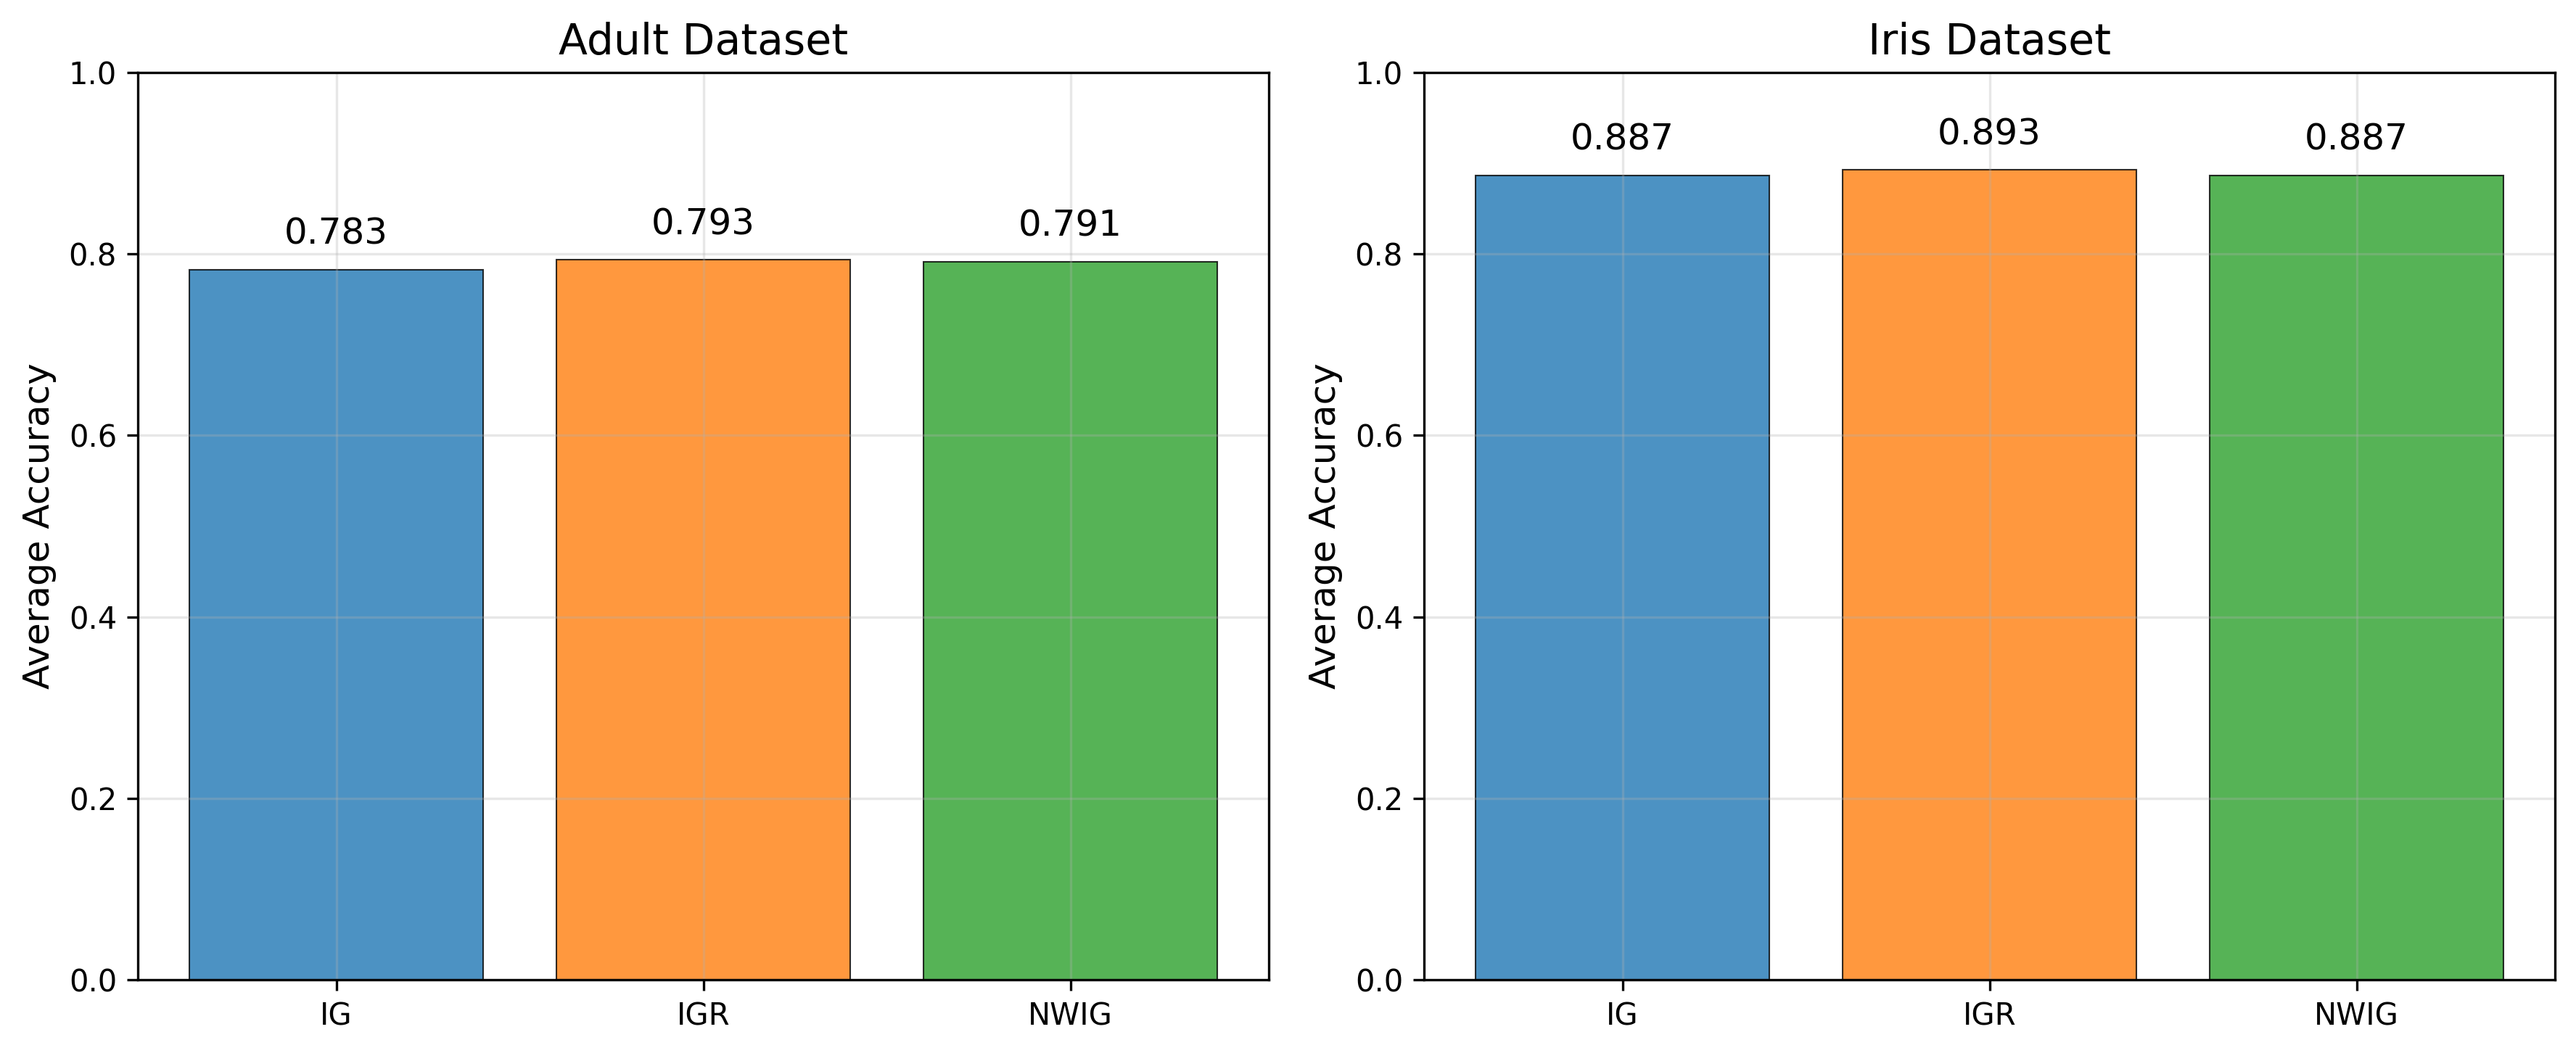
\includegraphics[width=0.8\textwidth]{accuracy_by_criterion.png}
    \caption{Accuracy comparison across different splitting criteria}
    \label{fig:accuracy_criterion}
\end{figure}

The results show that different criteria perform differently on different datasets. Information Gain Ratio (IGR) generally provides more stable performance by avoiding bias toward attributes with many values.

\subsection{Effect of Tree Depth}
Figure \ref{fig:accuracy_depth} demonstrates how tree depth affects classification accuracy.

\begin{figure}[H]
    \centering
    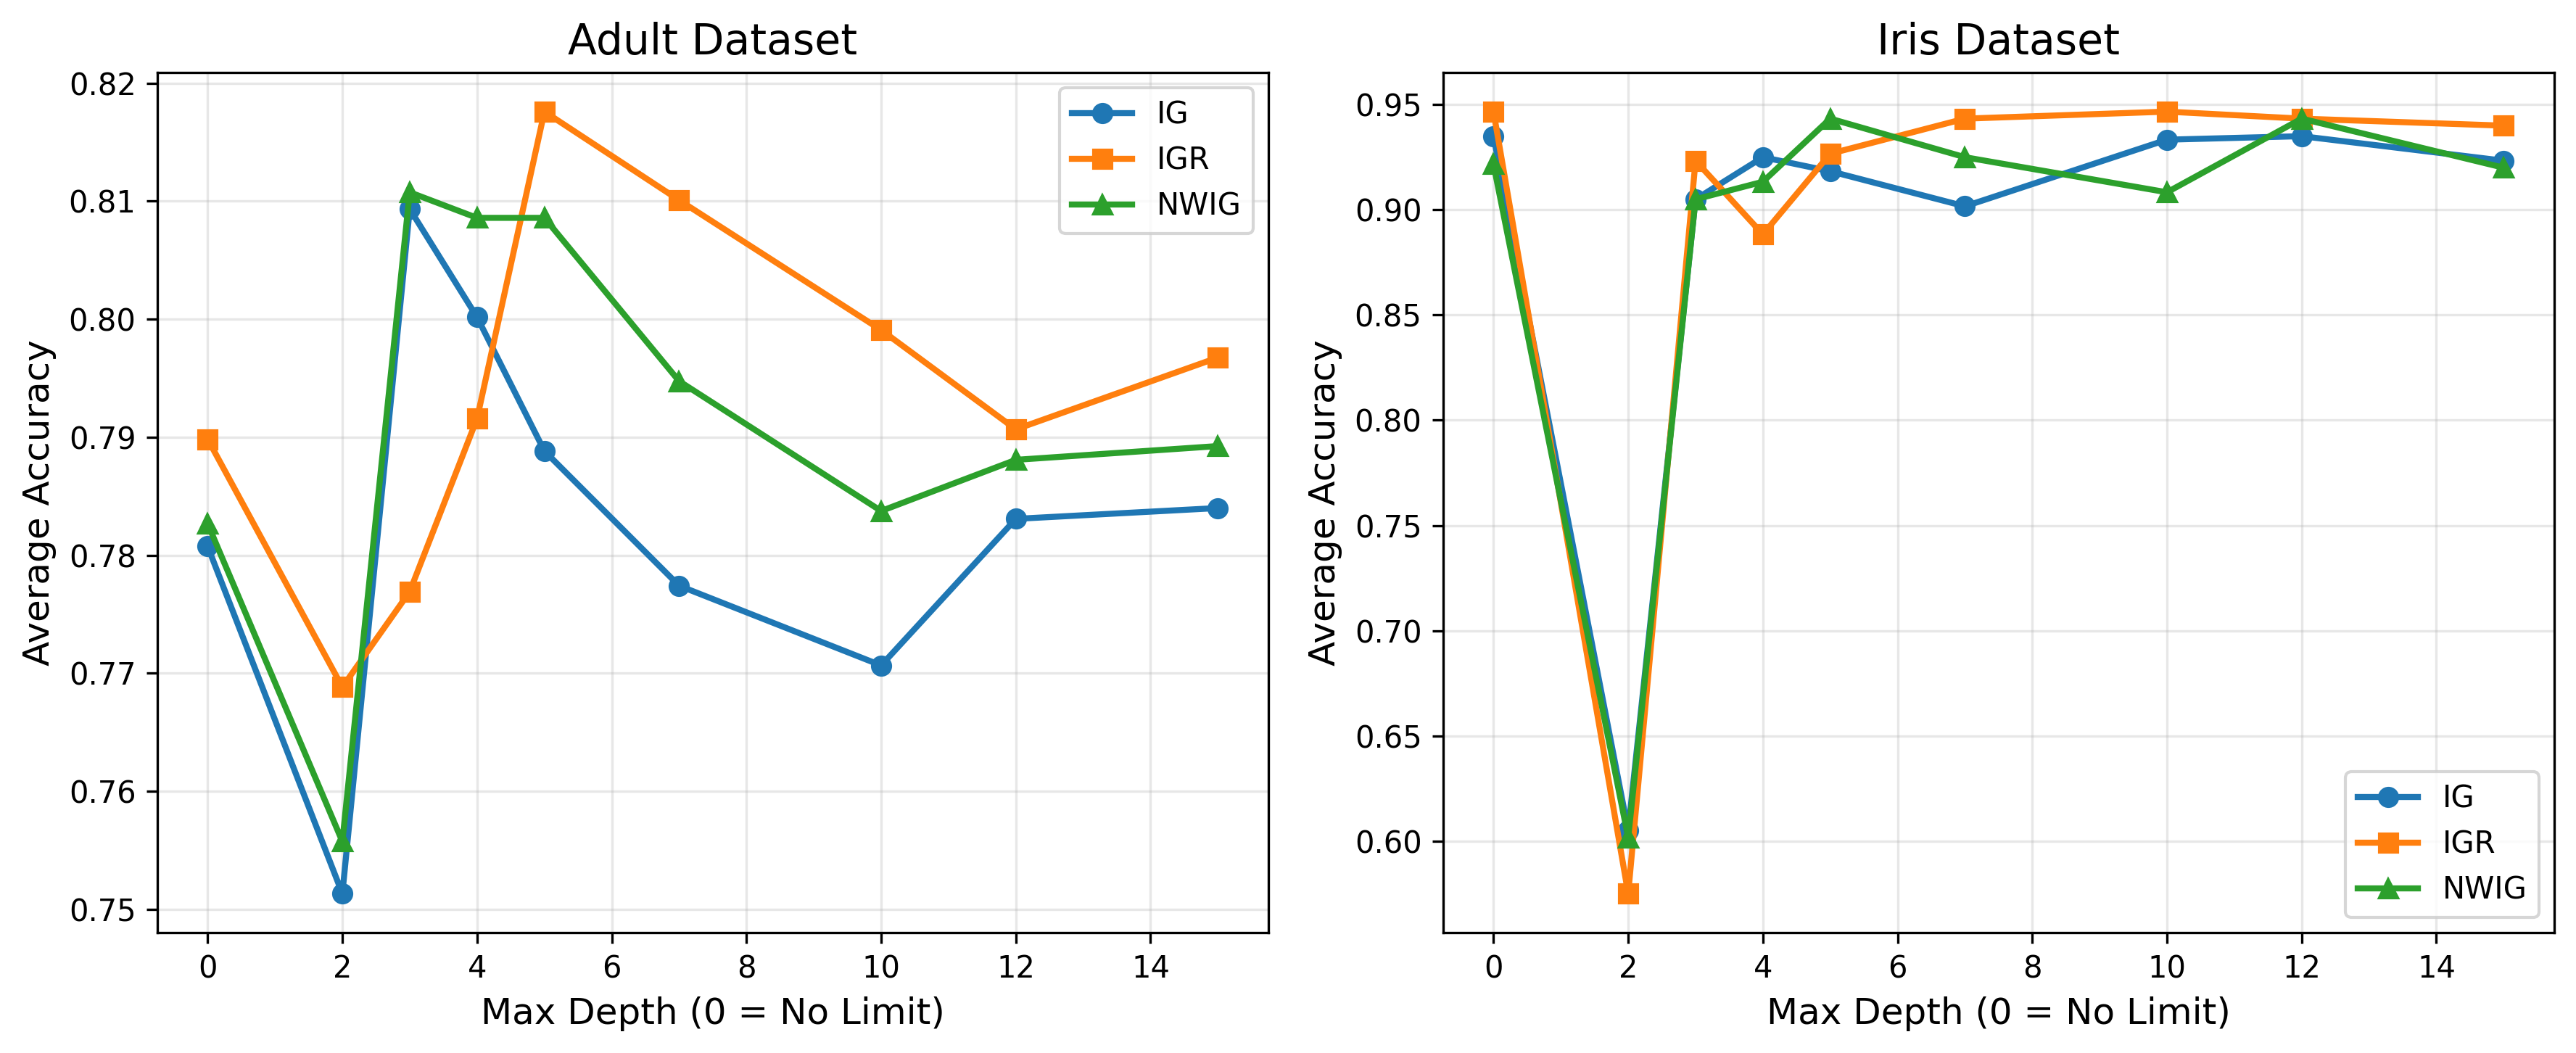
\includegraphics[width=0.8\textwidth]{accuracy_by_depth.png}
    \caption{Accuracy vs Tree Depth}
    \label{fig:accuracy_depth}
\end{figure}

The analysis reveals that deeper trees generally achieve higher accuracy up to a certain point, after which overfitting may occur.

\subsection{Depth Effect Analysis}
Figure \ref{fig:depth_analysis} provides a detailed view of how depth affects performance across different criteria.

\begin{figure}[H]
    \centering
    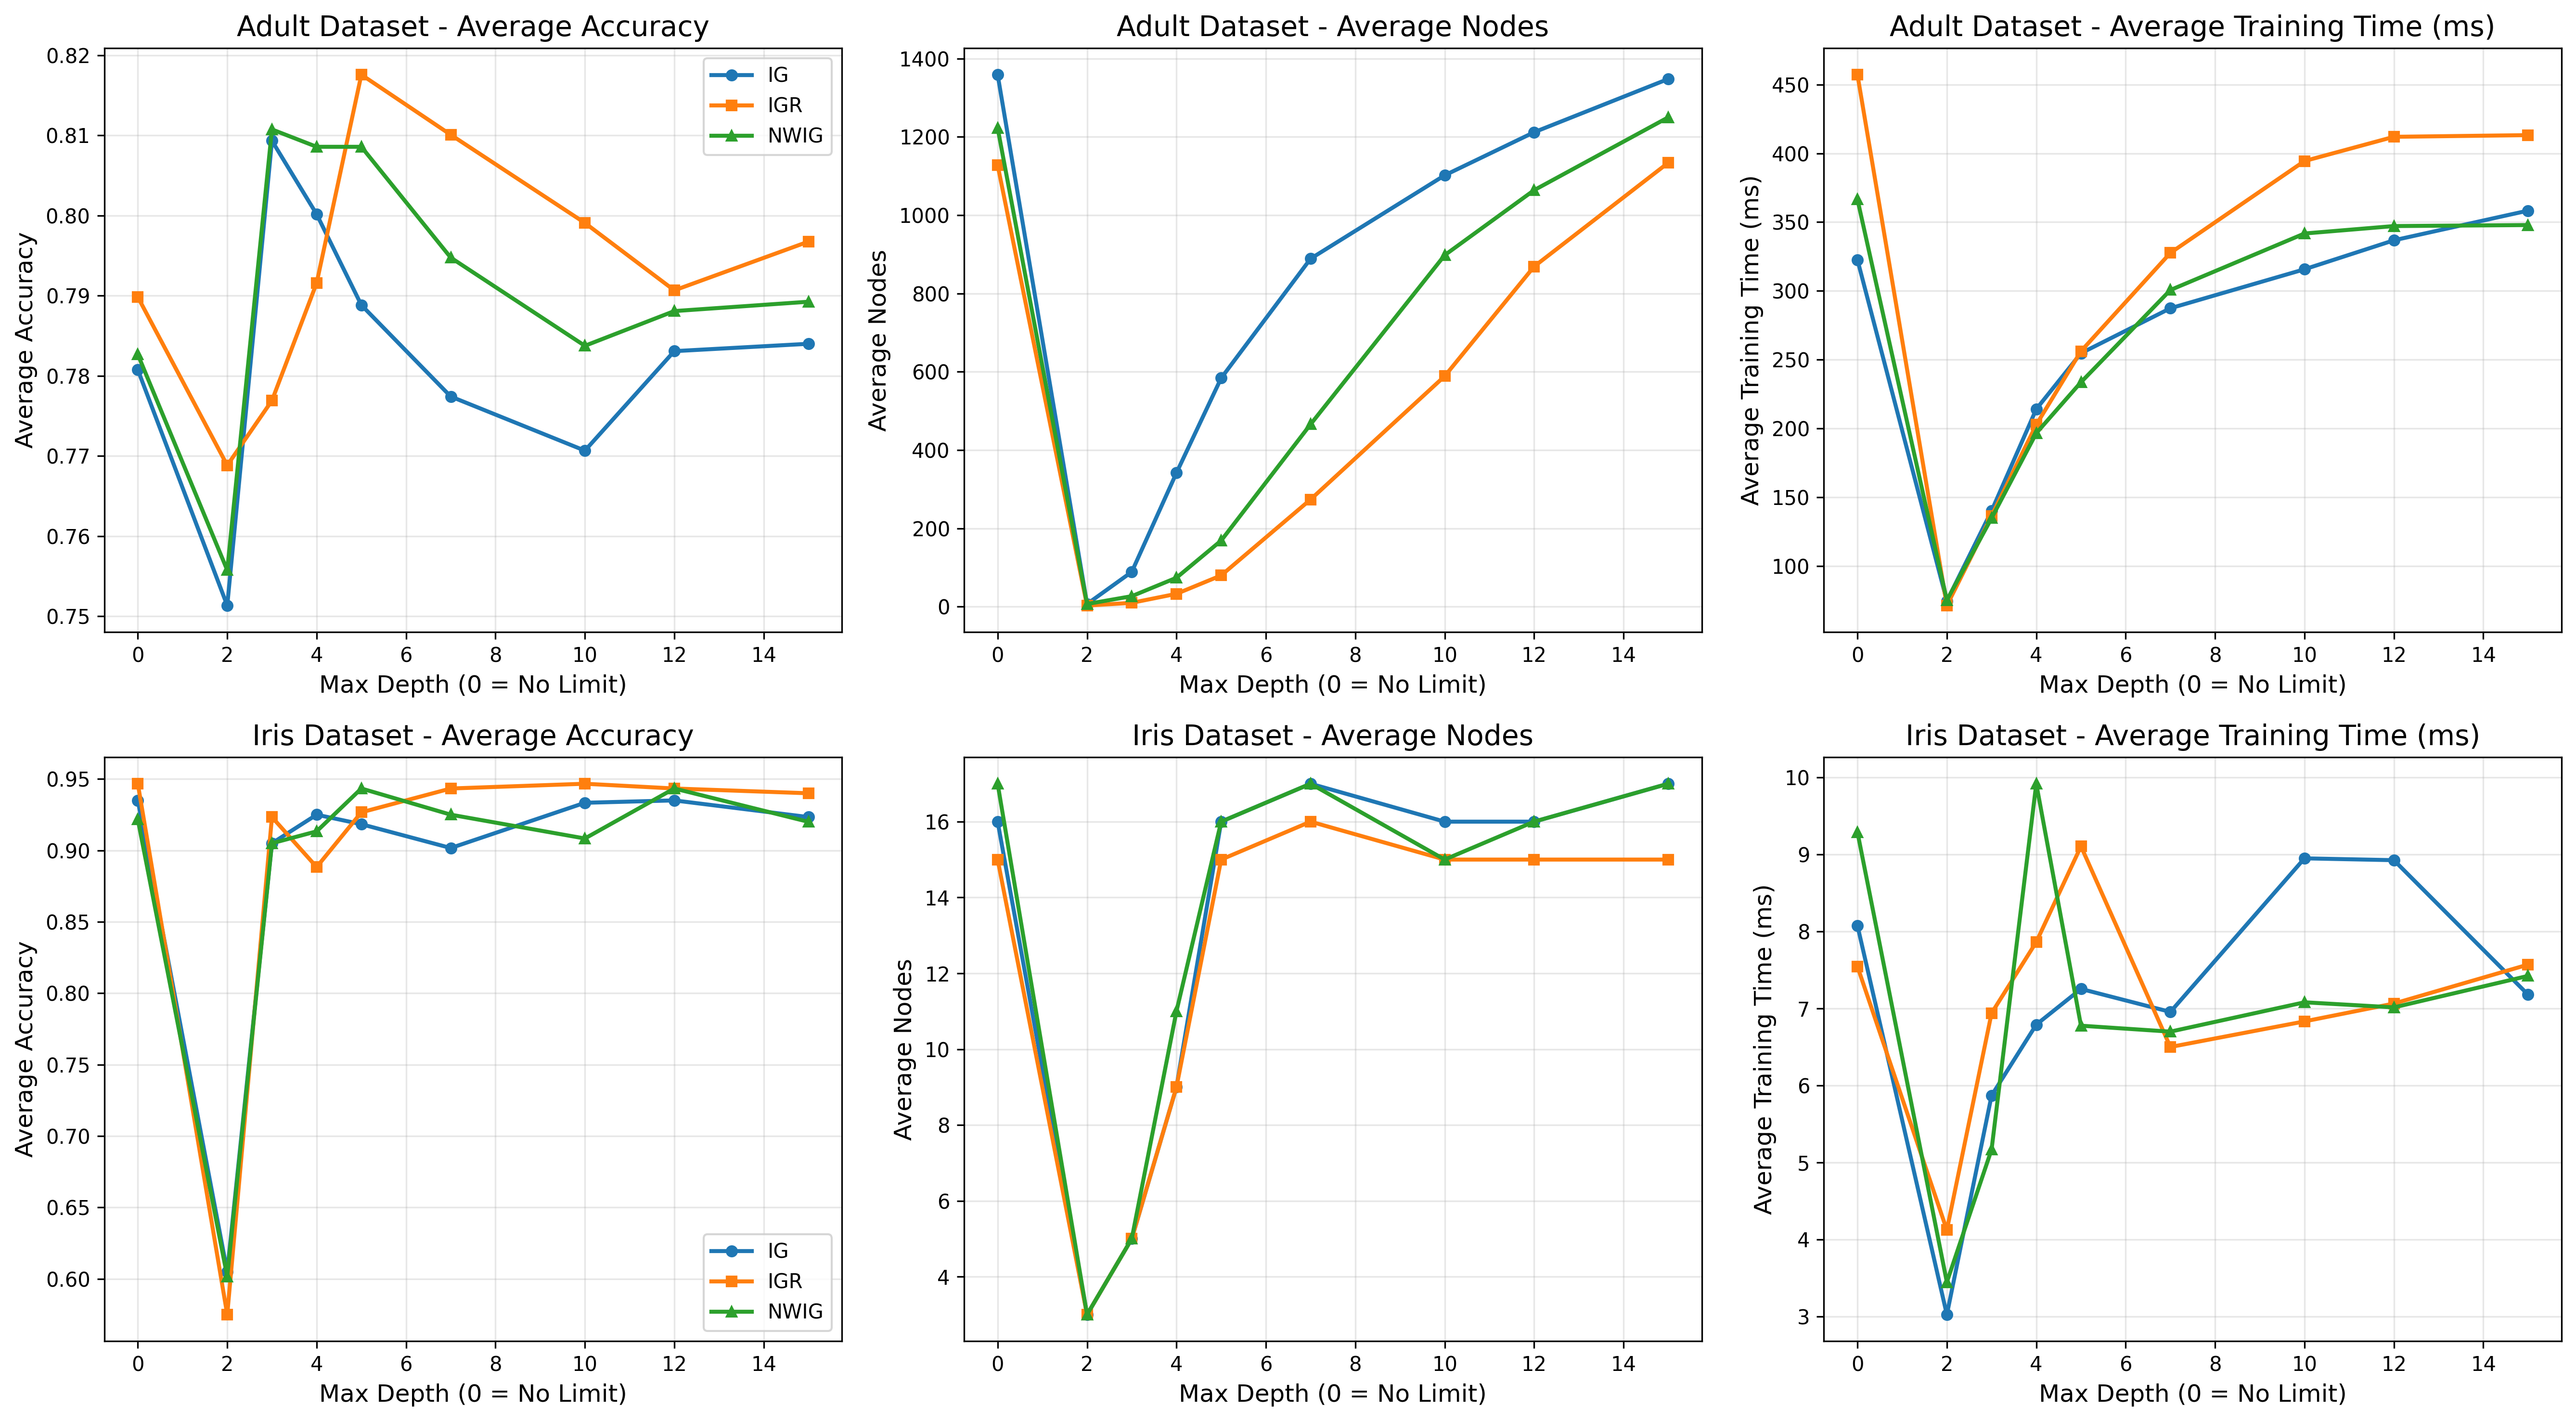
\includegraphics[width=0.8\textwidth]{depth_effect_analysis.png}
    \caption{Detailed depth effect analysis}
    \label{fig:depth_analysis}
\end{figure}

\subsection{Complexity vs Accuracy Trade-off}
Figure \ref{fig:complexity_accuracy} shows the relationship between tree complexity and accuracy.

\begin{figure}[H]
    \centering
    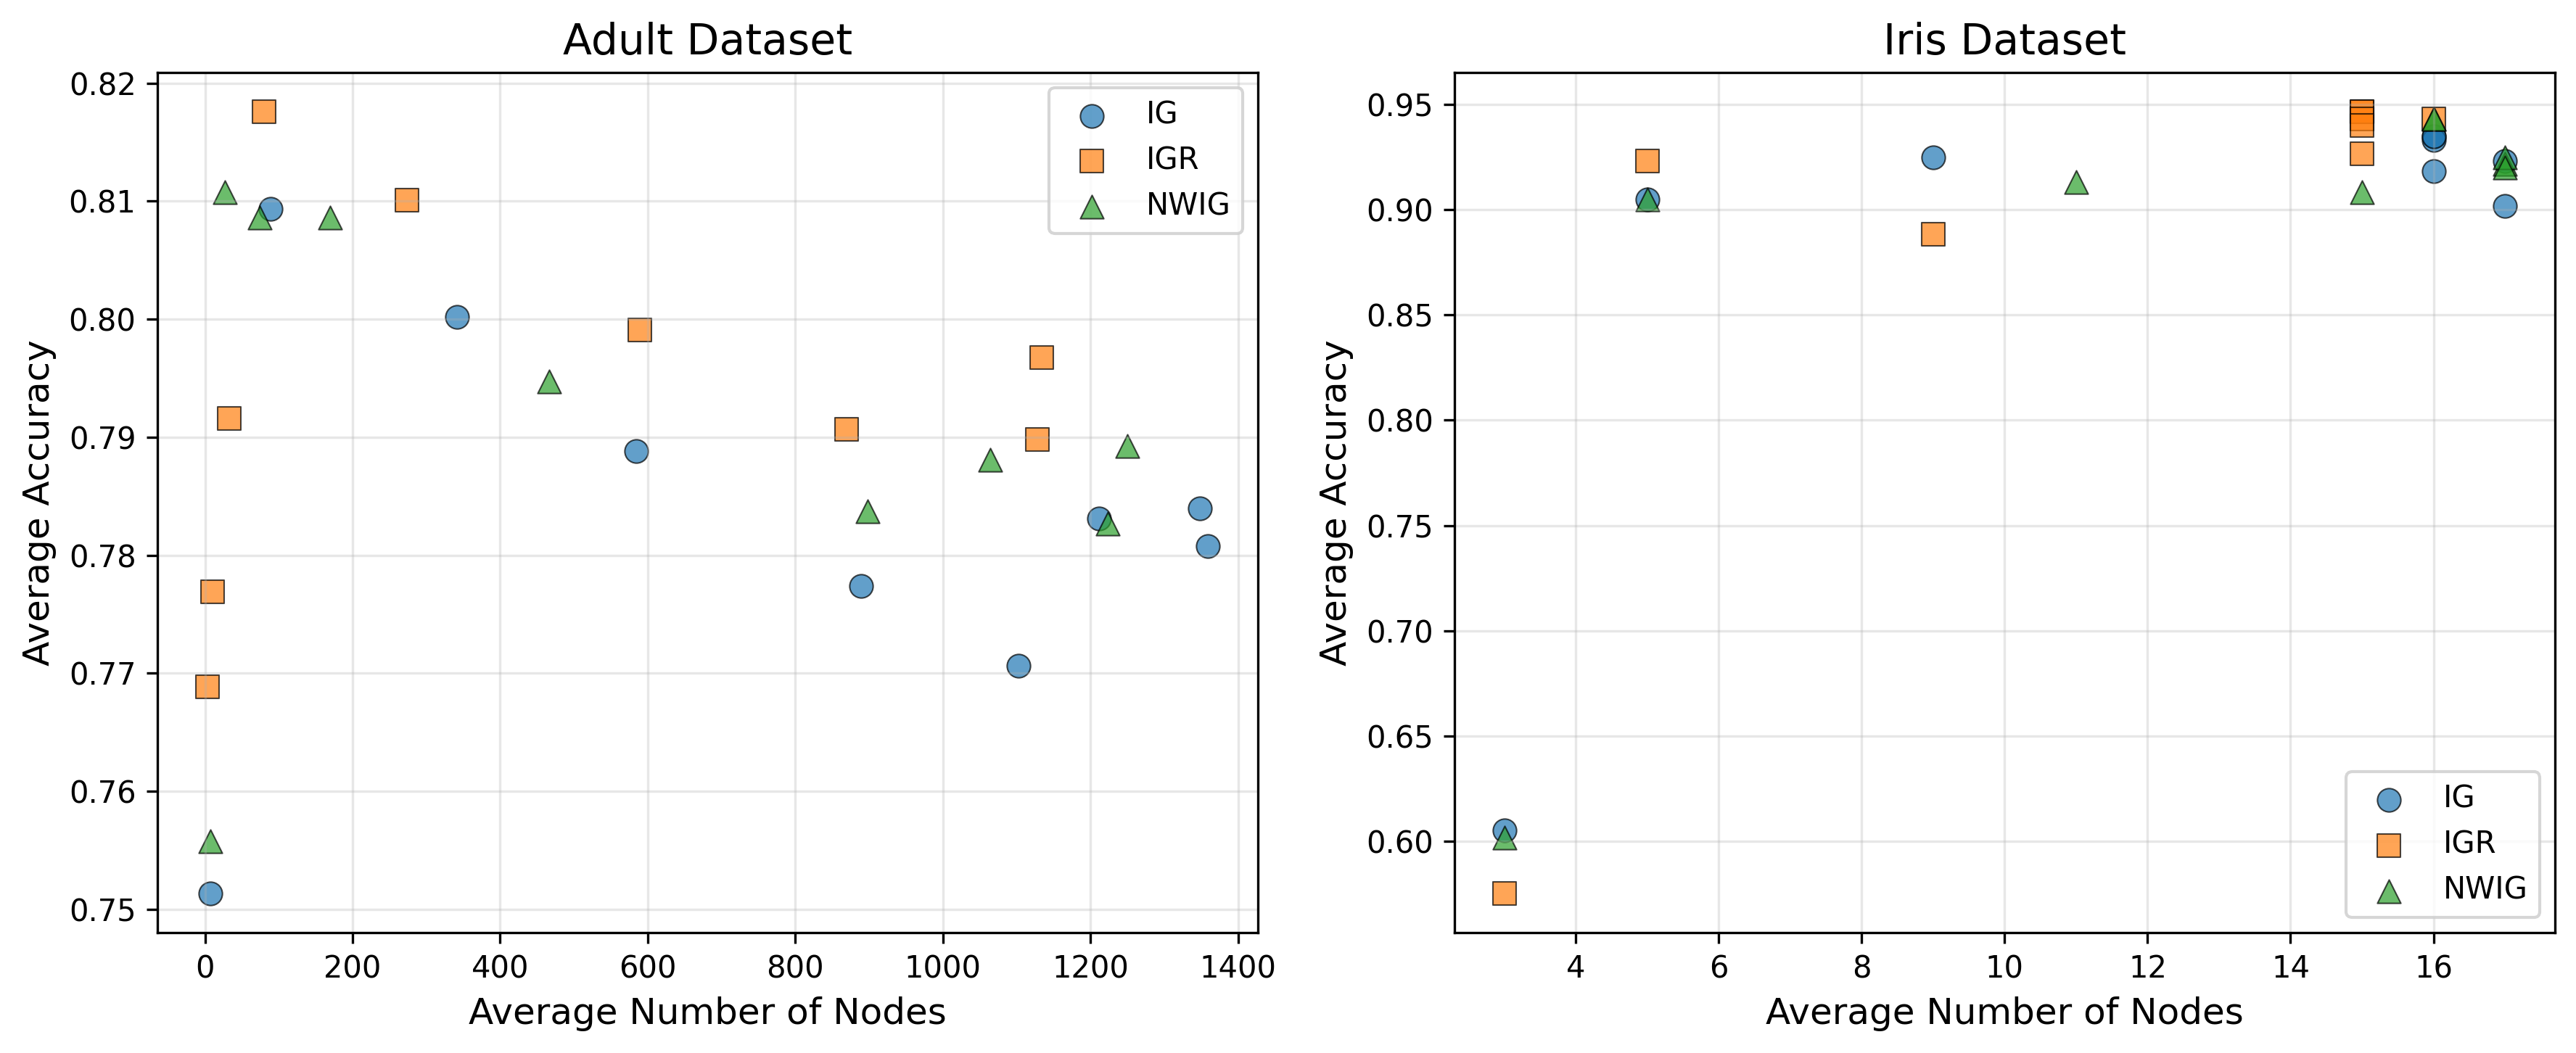
\includegraphics[width=0.8\textwidth]{complexity_vs_accuracy.png}
    \caption{Tree complexity vs accuracy trade-off}
    \label{fig:complexity_accuracy}
\end{figure}

This analysis helps identify the optimal balance between model complexity and performance.

\subsection{Performance Heatmap}
Figure \ref{fig:heatmap} provides a comprehensive view of performance across different parameters.

\begin{figure}[H]
    \centering
    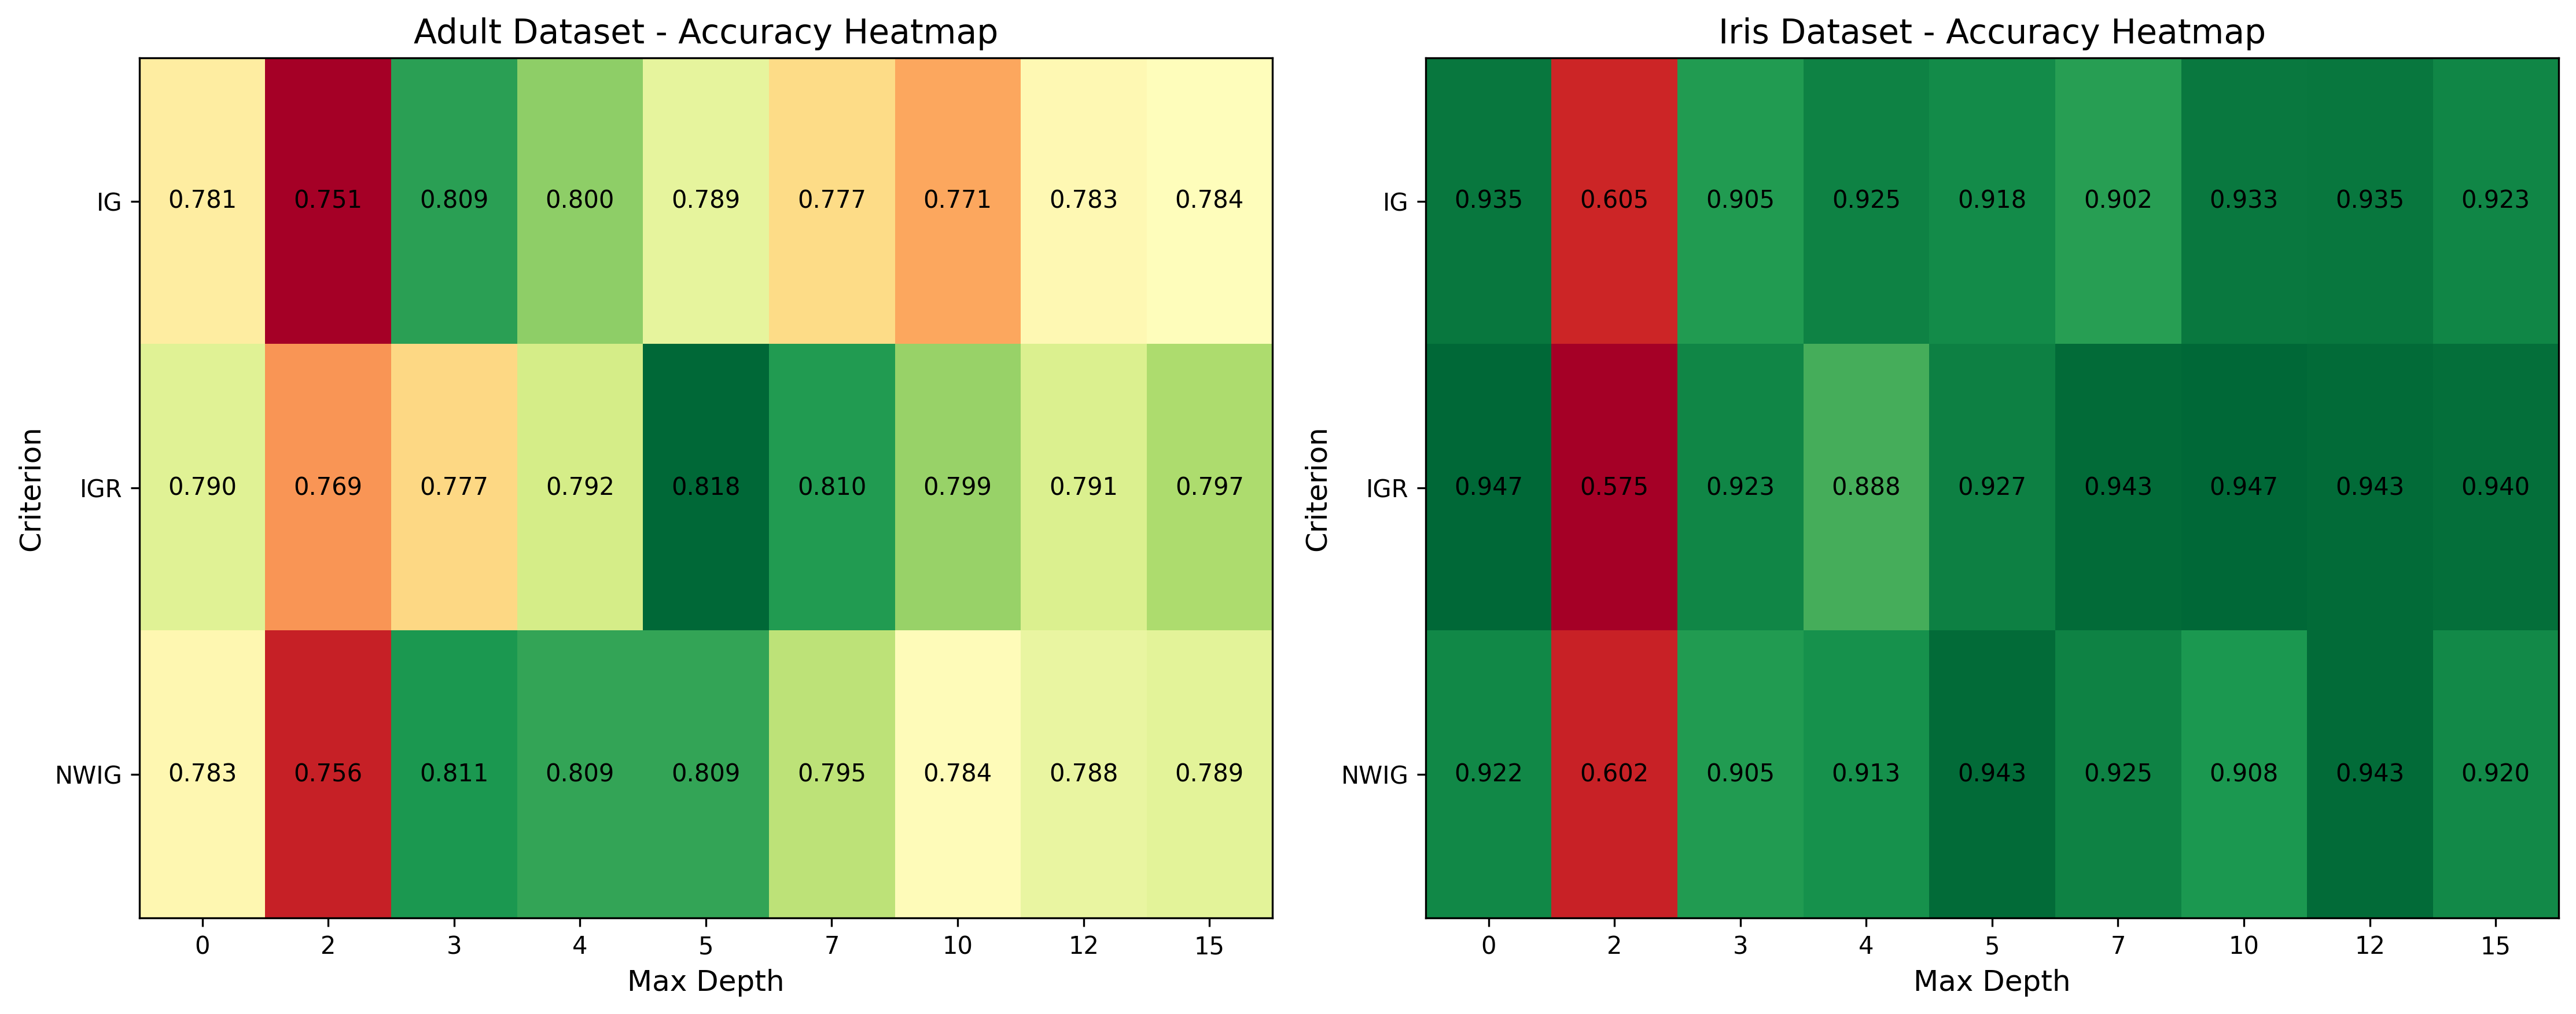
\includegraphics[width=0.8\textwidth]{performance_heatmap.png}
    \caption{Performance heatmap across different configurations}
    \label{fig:heatmap}
\end{figure}

The heatmap visualization makes it easy to identify optimal parameter combinations.

\subsection{Training Time Analysis}
Figure \ref{fig:training_time} shows the computational cost of different configurations.

\begin{figure}[H]
    \centering
    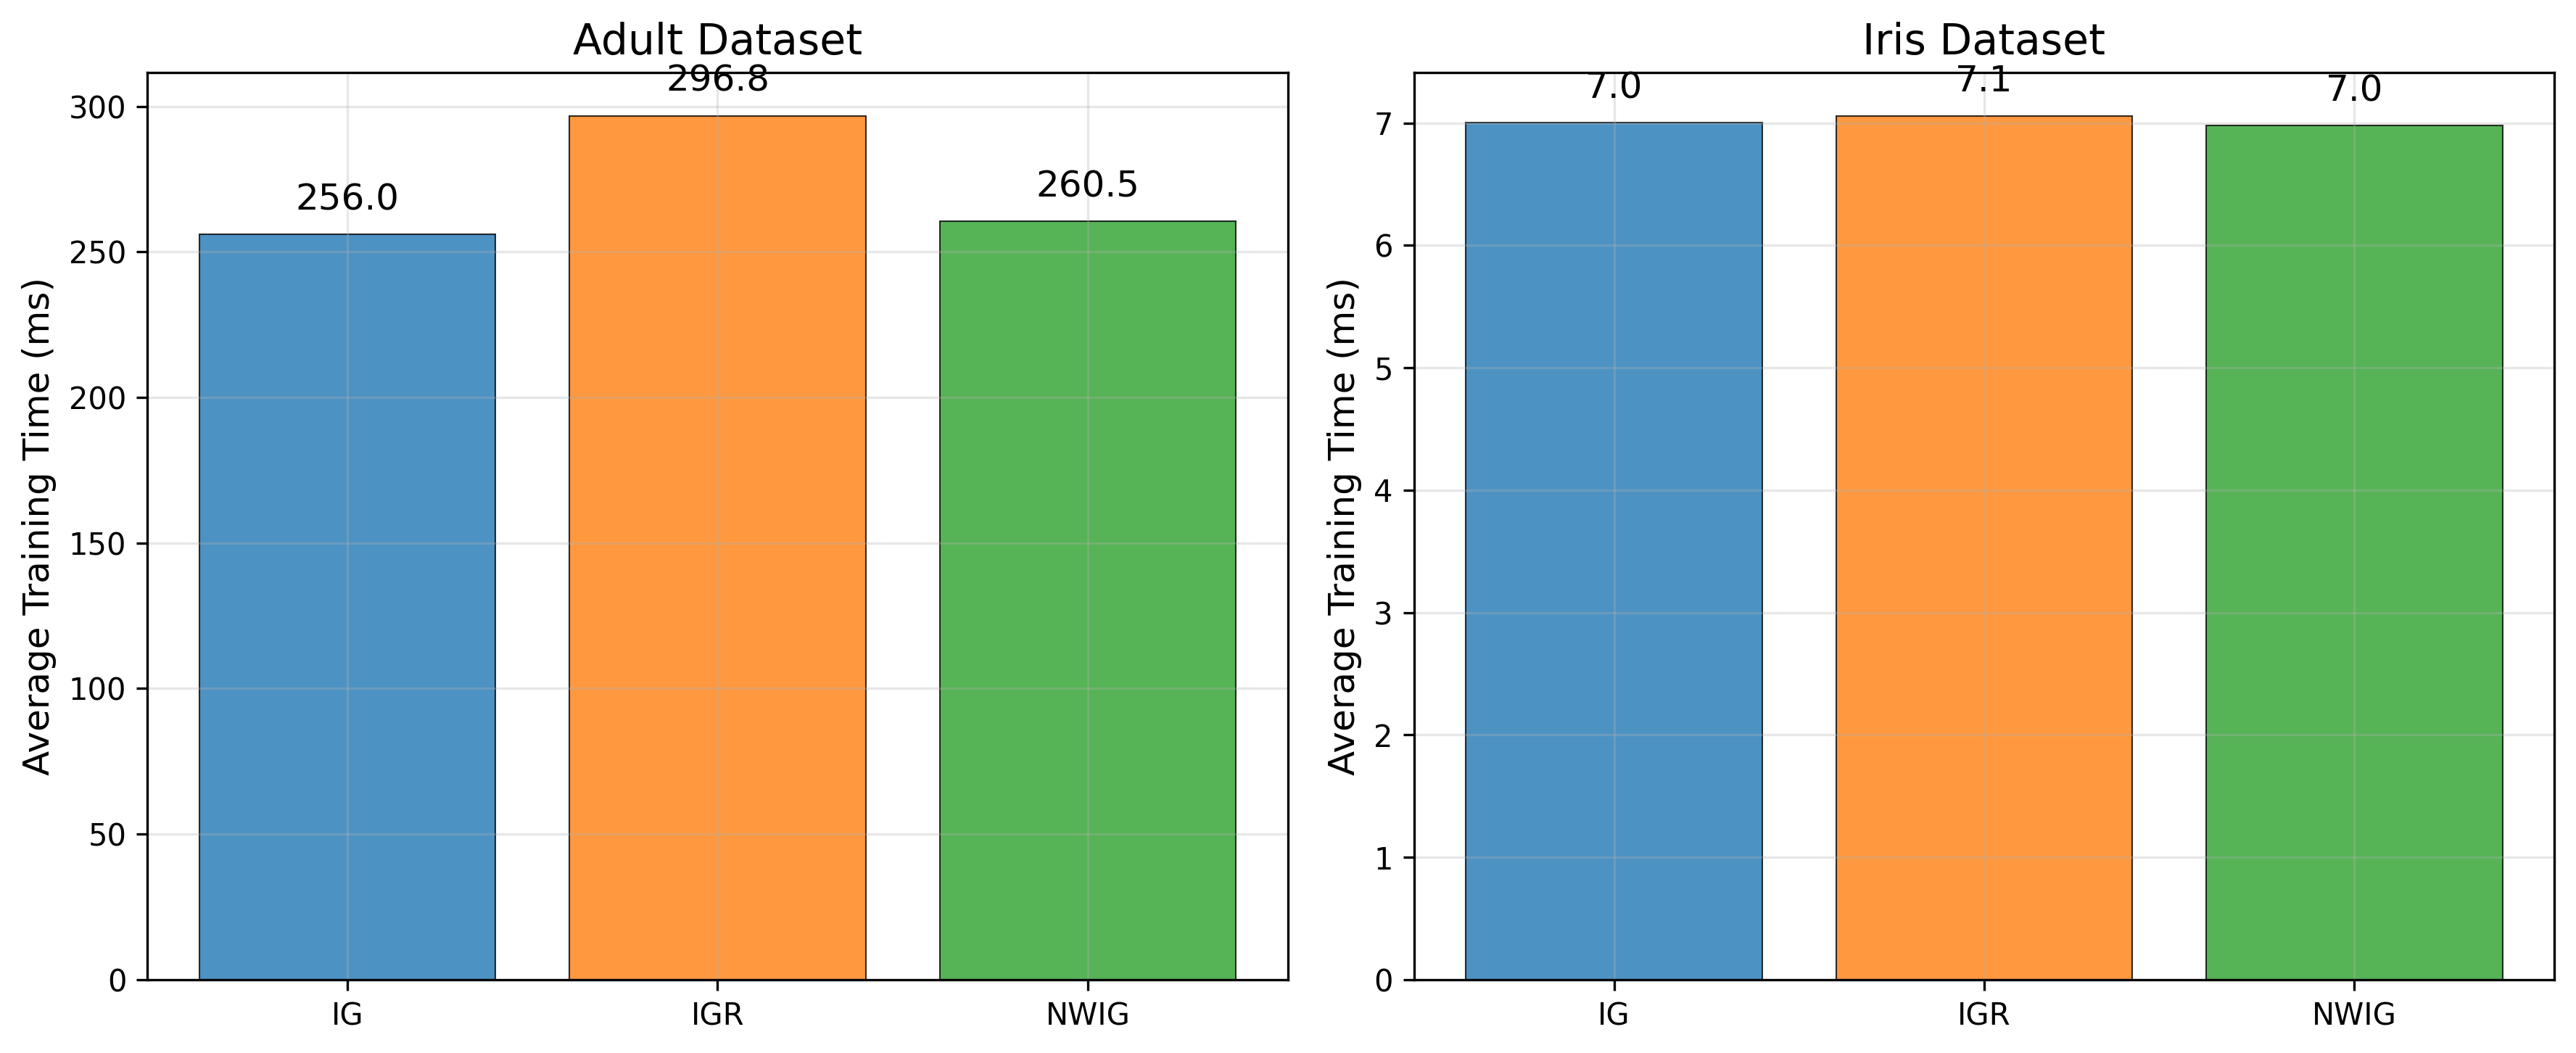
\includegraphics[width=0.8\textwidth]{training_time.png}
    \caption{Training time comparison}
    \label{fig:training_time}
\end{figure}

Training time is an important consideration for practical applications, especially with larger datasets.

\section{Key Findings}
\begin{enumerate}
    \item Information Gain Ratio (IGR) generally provides the most balanced performance across different datasets
    \item Tree depth significantly affects accuracy, with optimal depth varying by dataset
    \item Missing value handling using mode replacement works effectively for both numerical and categorical attributes
    \item There is a clear trade-off between tree complexity and generalization performance
    \item NWIG criterion shows promising results for certain datasets
\end{enumerate}

\section{Conclusion}
The experimental analysis demonstrates that the implemented decision tree algorithm works effectively across different datasets and configurations. The choice of splitting criterion and tree depth should be based on the specific characteristics of the dataset and the desired balance between accuracy and complexity.

The visualizations clearly show the performance patterns and help in making informed decisions about parameter selection. Future work could include implementing pruning techniques to further optimize the trade-off between accuracy and model complexity.

\end{document}
